\section{The spatiotemporal reservation closure}
\label{sec:strc}
%% =====================================================================

This section produces only the rewritable occupancy set \(U\). It takes as input the reservation table \(R\) and the seed set \(\mathrm{Src}(\mathcal{D})\)
(Definition~\ref{def:seeds}), builds a dependency graph over occupancies, takes its transitive closure, and outputs \(U=\mathrm{Cl}(\mathrm{Src})\).
How vehicles are rerouted on \(U\) is the subject of Section~\ref{sec:repair}.

\subsection{Reservation dependency edges}
\label{sec:closure_def}

\begin{definition}[Reservation dependency graph]
\label{def:dep}
The vertices are the corridor occupancies in \(R\). A directed edge \(r\to r'\) means ``invalidating \(r\) may force \(r'\) to be rerouted''. The edges are of four kinds:
\begin{enumerate}[leftmargin=1.4em,itemsep=0.15em]
\item \textbf{Yield edges:} two occupancies of the same corridor by different vehicles whose time intervals overlap \emph{or abut as half-open intervals}
(\(r.t^e=r'.t^s\)); the edge points from the earlier entrant to the later one. Abutting is legal under exclusive semantics, but if the former is delayed, the latter must give way.
\item \textbf{Same-vehicle successors:} two occupancies of the same vehicle that are adjacent in time order.
\item \textbf{Same-job successors:} an edge from the occupancies of operation \(i\) of a job to those of operation \(i+1\) of the same job.
\item \textbf{Same-machine successors:} edges between the occupancies induced by two operations that are adjacent on the timeline of the same machine.
\end{enumerate}
This yields \(G_R=(R,E_R)\).
Figure~\ref{fig:graphs}(b) illustrates the four kinds of edges. Same-job successor edges connect the occupancies induced by consecutive operations,
and same-machine successor edges connect the occupancies induced by two operations adjacent on the timeline of one machine;
both have legs as endpoints, consistent with the granularity of Section~\ref{sec:shop}.
The four kinds of edges answer a single question: after \(r\) is rewritten, might \(r'\) have to be rewritten as well?
The edge set is a modeling choice; its completeness is tested by the difference probe of Section~\ref{sec:e3}.
\end{definition}

\begin{definition}[\STRC{}]
\label{def:strc}
Given a seed set \(S\subseteq R\), a horizon \(H\), and a time \(t_{\mathrm{now}}\),
denote the occupancies that are unfinished at the decision time and start before the horizon by
\[
R^{\circ}=\bigl\{\,r\in R:\ r.t^e>t_{\mathrm{now}},\ r.t^s<H\,\bigr\},
\]
and let \(G_R^\circ\) be the subgraph of \(G_R\) induced by \(R^{\circ}\).
The result of the spatiotemporal reservation closure, namely the reservation impact set, is defined as
\[
\mathrm{Cl}(S)
=\bigl\{\,v\in R^{\circ}:\
\exists\,s\in S\cap R^{\circ}\ \text{such that}\ s\!\to^*\!v\ \text{in}\ G_R^\circ\,\bigr\},
\]
that is, all unfinished occupancies reachable along outgoing edges from the unfinished seeds (the seeds themselves included).
All experiments in this paper use \(H=C_{\max}(\mathcal{S}^0)+1\). Then \(r.t^s<H\) holds for every occupancy in \(\mathcal{S}^0\)
and the horizon filters nothing; we keep \(H\) only so that the definition also applies to a rolling horizon.
If \(G_R^\circ\) is stored as adjacency lists (with edge set \(E_R^{\circ}\)), the set can be computed with a queue in
\(O(|R^{\circ}|+|E_R^{\circ}|)\) time. We did not time this step separately;
delineating the scope is only one component of the millisecond-range results of Section~\ref{sec:cheap}.
\end{definition}

Figure~\ref{fig:closure} gives an illustration: (a) the blockage window and the occupancies taken as seeds; (b) the dependency edges and the boundary of the reservation impact set.
No occupancy outside the set is an outgoing-edge successor of an occupancy inside it (Proposition~\ref{prop:struct}).

\begin{figure}[t]
\centering
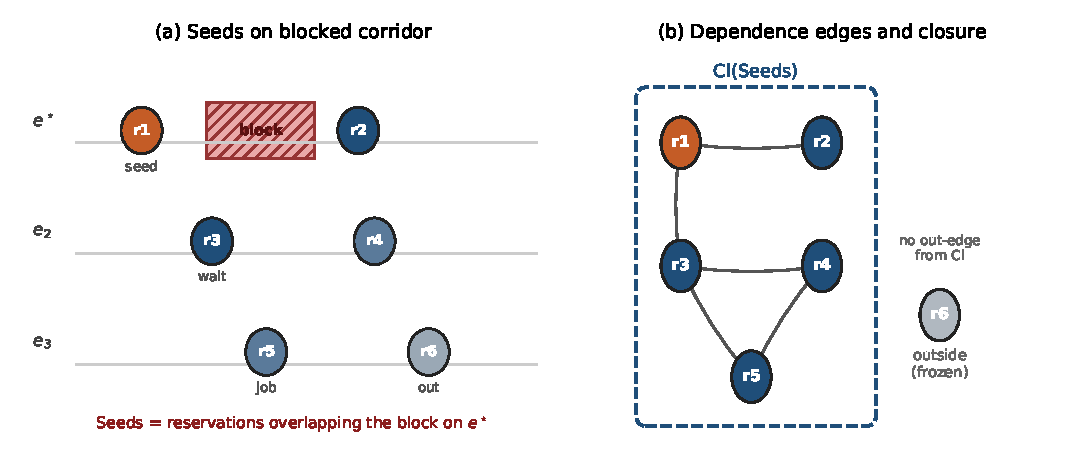
\includegraphics[width=\linewidth]{figures/fig_strc_closure}
\caption{Construction of the reservation impact set.
(a)~Occupancies that overlap the corridor blockage window serve as seeds;
(b)~taking the transitive closure along the four kinds of dependency edges (yielding, plus the same-vehicle, same-job, and same-machine succession relations) yields
\(\mathrm{Cl}(\mathrm{Src})\); occupancies outside the set are kept as planned.}
\Description{Two small panels. (a) On a space--time diagram, a blockage window covers several occupancies,
which are marked as seeds. (b) The transitive closure along directed dependency edges from the seeds gives the boundary of the reservation impact set;
occupancies beyond the boundary have no incoming edges from inside the set and are kept as planned.}
\label{fig:closure}
\end{figure}

The baseline that scopes on the operation-precedence graph maps \(T_{\mathrm{impact}}\) to rewritable occupancies:
all occupancies whose task label belongs to the affected set and whose \(t^e>t_{\mathrm{now}}\).
By Proposition~\ref{prop:miss}, this set is empty under Class B disturbances.
Scoping on the reservation impact set takes \(U=\mathrm{Cl}(\mathrm{Src})\).
In the experimental tables the two are denoted R1 and R2, respectively.

\subsection{Containment}
\label{sec:containment}

\begin{prop}[Structural closure]
\label{prop:struct}
For any \(S\subseteq R\), \(G_R^\circ\) contains no edge
\(u\to v\) with \(u\in\mathrm{Cl}(S)\) and \(v\in R^{\circ}\setminus\mathrm{Cl}(S)\).
Consequently, no unfinished occupancy outside the impact set is reachable along outgoing edges from \(\mathrm{Cl}(S)\).
\end{prop}

\begin{proof}
Suppose such an edge \(u\to v\) exists. Since \(u\in\mathrm{Cl}(S)\), there is an unfinished seed \(s\) with
\(s\to^* u\). Appending \(u\to v\) gives \(s\to^* v\), so \(v\in\mathrm{Cl}(S)\) by Definition~\ref{def:strc},
a contradiction.
\end{proof}

Proposition~\ref{prop:struct} shows that ``local'' corresponds to a graph-theoretically closed object: no occupancy outside the impact set is a direct successor of
any occupancy inside it. Once the edge set is fixed, closure is a corollary of the definition; its physical completeness depends on how the edge set is chosen.

\begin{remark}[The reservation impact set and the minimal rewritable set]
\label{rem:minimality}
Structural closure states only that the impact set is closed under the modeled dependency edges: no dependency edge leads from inside the set to outside it.
It neither guarantees that the impact set suffices to restore feasibility nor shows that the impact set is not too large. For the latter there are three reasons.

First, \textbf{the minimal rewritable set depends on the repair procedure used, whereas the reservation impact set does not}.
To call a set \(U\) minimal, one must specify ``under which repair capability \(U\) suffices to restore feasibility''. The minimal \(U\) when reassignment and resequencing are allowed
differs from the minimal \(U\) when only rerouting is allowed. The reservation impact set is uniquely determined by \(G_R\) and independent of the repair procedure.
Hence, by definition, it is not tied to any particular heuristic, and it cannot simultaneously be a procedure-dependent minimal set.

Second, \textbf{the four kinds of edges admit occupancies that need not be rewritten, while the known case of missed occupancies, abutting, has been folded into the yield edges}.
Yield edges are built on ``same corridor, different vehicles, overlapping or abutting'': any overlap creates an edge, without checking whether the latter \emph{truly}
can proceed only by waiting for the former to pass. If a bypass exists there, the latter can simply detour and need not enter the rewritable set. Likewise, same-vehicle successor edges
may pull in chain tails that the delay cannot reach. Both effects make the impact set larger than necessary.
In the opposite direction, half-open intervals that meet end to start (abutting) are legal under exclusive semantics, but if the former is delayed the latter must give way;
abutting is therefore also connected by yield edges. The difference probe finds \ProbeLeaks\ leaks over \(\NPairs\) pairs (\ProbeLeakPairs;
Section~\ref{sec:limitations}). This test targets the known abutting omission and does not prove the edge set complete.

Third, \textbf{empirically, the impact set is not small}. Section~\ref{sec:e6} reports that under corridor blockage the reservation impact set covers on average about
\ClosureAliveFrac\ of the occupancies still unfinished after \(t_{\mathrm{now}}\). Relative to the trivial upper bound of ``rewriting every occupancy unfinished at the decision time'',
the impact set leaves out less than one tenth. The savings of bounded repair come mainly from \emph{not rewriting finished occupancies} and \emph{not restarting the search},
not from a sharp reduction of the future occupancies to be rewritten; ``local'' and ``bounded'' do not mean that the changes are small.

``Less than one tenth'' is a ratio of the \emph{sizes} of rewritable sets, not a difference in rewrite fraction.
Section~\ref{sec:cheap} measures the trivial upper bound above as a separate baseline (RA) and finds that this very difference of less than one tenth
lowers the rewrite fraction from \ResFracAllFuture\ to \ResFracCheapRtwo\ (per cell \RAStabWTL,
\(p=\RAStabP\)), while runtime and makespan remain nearly unchanged.

What this paper provides, therefore, is a rewritable set that is uniquely determined by structure, reproducible, and closed under the dependency edges,
and that sufficed to restore feasibility in all our experiments. Approximating the minimal rewritable set is a separate problem, left for future work
(Section~\ref{sec:future}).
\end{remark}

\begin{prop}[A sufficient condition for unchanged fields outside the set]
\label{prop:outside}
Let the rewritable occupancy set be \(U=\mathrm{Cl}(S)\), and let level-1 rerouting be executed as in Section~\ref{sec:level1}:
(i)~the no-entry windows have been written into the routing layer; (ii)~for every \(r\in R^{\circ}\setminus U\), its original fields
\((e,[t^s,t^e),k)\) are pre-committed to the new reservation table and the pre-commit succeeds;
(iii)~the router is invoked to generate new occupancies only for transports in \(U\); (iv)~the final schedule passes the conflict-free check.
Then, in the recovered reservation table \(R'\), the corridor, interval, and vehicle of every \(r\in R^{\circ}\setminus U\) agree with
\(\mathcal{S}^0\). The quantifier here ranges over \emph{occupancies}, not tasks: a transport may have some occupancies in \(U\)
and others outside it, in which case only the part outside the set is protected by this proposition.
\end{prop}

\begin{proof}
By (ii), the occupancies outside the set are written into the new table with their original intervals before the replay begins, and they do not conflict with the no-entry windows
(otherwise the pre-commit would fail). Step (iii) commits new occupancies only for tasks in \(U\) and neither deletes nor rewrites the committed
intervals outside the set. Hence, for task labels outside the set, \((e,[t^s,t^e),k)\) in the new table equals the pre-committed value,
and thus equals the value in \(\mathcal{S}^0\). Passing the check only rules out conflicts between new and existing occupancies; it does not alter committed fields.
\end{proof}

Premises (i)--(iv) are execution conditions of the rerouting procedure in Section~\ref{sec:level1} and can be verified against the algorithm one by one.
They differ in kind from model-level assumptions such as A1--A5, so we do not add them to the numbered assumptions. Beyond them, the proposition relies on
A1 (the initial schedule is feasible; otherwise the original fields outside the set might conflict with one another and the pre-commit would necessarily fail),
A2 (finished occupancies are not revisited), and A4 (corridors are exclusive).

\begin{remark}[How premises (ii) and (iii) can each fail]
\label{rem:precommit}
If the pre-commit fails because ``an occupancy outside the set overlaps a no-entry window'', then \(S\) does not cover all occupancies overlapping the blockage window, and the seed set is incomplete.
If rerouting fails at a transport--operation hand-off and triggers the scope escalation of Section~\ref{sec:scope_escalation}, the new rewritable set satisfies
\(U'\supsetneq U\), and Proposition~\ref{prop:outside} holds only for the occupancies that are ultimately left outside the rewritable set.
Scope escalation puts feasibility ahead of minimal rewriting and is reported separately in the experiments.
One further failure lies outside what the proposition controls but occurs easily in implementations: premise (iii) requires the router to generate new occupancies \emph{only}
for transports in \(U\). If an implementation decides whether to reroute at a unit coarser than an occupancy (e.g., a whole transport or a whole operation),
occupancies outside \(U\) are rewritten along with it, premise (iii) no longer holds, and the conclusion of the proposition fails.
Remark~\ref{rem:e2b_history} records an instance of this in our implementation and its fix.
\end{remark}

\subsection{Structural predictability}
\label{sec:structure}

The size of the reservation impact set is uniquely determined by \(G_R\); once the schedule and network are given, there is no tunable parameter. Section~\ref{sec:instscale} scales the instances from \(8\times4\times4\) up to
\(\ScaleJobsHi\times\ScaleMachHi\times\ScaleMachHi\); the impact-set share fluctuates between
\ScaleCloLo\ and \ScaleCloHi\ and does not rise with size (this share uses the full table as denominator, with an attainable upper bound of about
\ScaleAliveShare; with the rewritable-eligible set as denominator it is \ScaleCloAliveLo--\ScaleCloAliveHi).
Hence the extent of ``local'' is measurable, but its size is not small (Remark~\ref{rem:minimality}).

As for \emph{which} structure corresponds to a larger impact set, the experimental result is negative.
We examine a class of indicators computed from the network alone and independent of the current schedule: the minimum number of corridors that must be cut to separate the load/unload stations from the rest of the shop,
i.e., the LU minimum cut (hereafter the LU cut), together with the funnel share; we refer to this family of indicators as static cuts below.
\textbf{The impact-set size is not determined by static cuts}. On our own layouts of the same size, under different boundary-blockage protocols, the
relative size either falls within a very narrow band or shows a direction but with values heavily overlapping across random seeds. On a batch of networks not designed by us,
the LU cut and the funnel share are \emph{constant}, whereas the impact-set share changes markedly across three machine configurations on the same network
(\(6\), \(7\), and \(8\) machines). A constant indicator cannot explain a varying quantity
(Section~\ref{sec:e4}).
This negative result concerns static cuts only; because few public networks are available, the general relation between network structure and impact-set size remains undetermined.
The next candidate characterization should be a schedule-dependent quantity rather than a purely topological one (Section~\ref{sec:future}).

%% =====================================================================
\section{Bounded repair on the reservation impact set}
\label{sec:repair}
%% =====================================================================

Figure~\ref{fig:framework} outlines the procedure of this section. We first delineate the rewritable occupancy set \(U\) by the reservation impact set,
then reroute only the transports inside the set while keeping occupancies outside it as planned; if the result is still infeasible, we escalate \(U\) and retry.
The baseline that scopes on the operation-precedence graph replaces only the source of \(U\); the global rescheduling baseline searches anew within a time limit.
All methods share the same corridor network, time-window routing, and conflict-free check.

\begin{figure}[t]
\centering
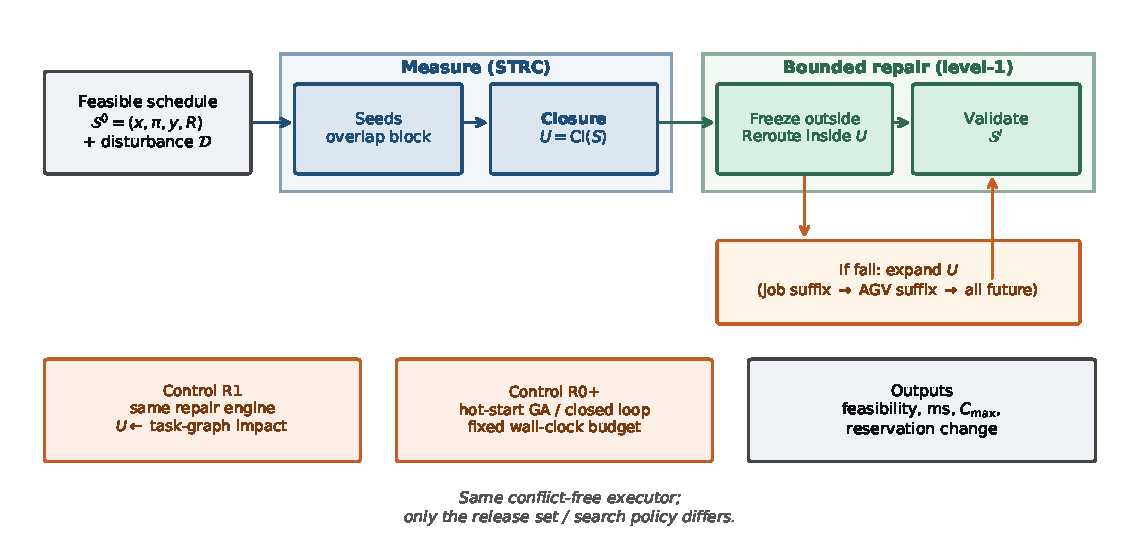
\includegraphics[width=\linewidth]{figures/fig_strc_framework}
\caption{Bounded repair scoped on the reservation impact set.
Top row: the impact set is obtained from the seeds and vehicles are rerouted; middle row: the rewritable scope is escalated after failure;
bottom row: the baseline scoping on the operation-precedence graph, the warm-started global rescheduling baseline, and the output metrics.
The figure shows only the three method-level paths; three further baselines operate within the millisecond range (Section~\ref{sec:cheap}).}
\Description{A three-row flowchart. Top row: after a disturbance arrives, the reservation impact set is obtained from the seeds; occupancies inside the set are rewritable,
those outside are kept as planned, and the original vehicles are rerouted. Middle row: when rerouting fails, the rewritable set is escalated in the order job suffix, same-vehicle suffix,
all unfinished occupancies, and the rerouting is retried. Bottom row: two baselines,
one scoping by the affected set on the operation-precedence graph and one performing a warm-started global search; the three paths feed the same set of output metrics.}
\label{fig:framework}
\end{figure}

\subsection{Rewritable set, kept-as-planned set, and level-1 rerouting}
\label{sec:level1}

Given the rewritable occupancy set \(U\), level-1 rerouting keeps the original vehicle and machine assignments and replays in the original processing order.
Rerouting operates at the granularity of corridor segments (a segment is the portion of one trip that traverses a single corridor). Segments a vehicle has already traversed before
\(t_{\mathrm{now}}\) are finished occupancies and are pre-committed unchanged; rerouting plans only from the node where the vehicle is at that time.
A granularity coarser than segments would rewrite finished occupancies (Remark~\ref{rem:e2b_history}).
Algorithm~\ref{alg:replay} gives this primitive; Algorithm~\ref{alg:strc_repair} wraps it, computing the reservation impact set and escalating \(U\) on failure.

\begin{algorithm}[t]
\caption{Level-1 rerouting replay \(\textsc{ReplayReroute}\)}
\label{alg:replay}
\begin{algorithmic}[1]
\Require schedule \(\mathcal{S}^0=(x,\pi,y,R)\), disturbance \(\mathcal{D}\), rewritable set \(U\), time \(t_{\mathrm{now}}\)
\Ensure schedule \(\mathcal{S}'\) or failure
\State write \(\mathcal{D}\) into the routing layer
  \Comment{blockage: no-entry window; slowdown: overlapping portion \(\tau\)}
\State take an empty table \(R'\)
\For{each non-rewritable occupancy: all those outside the set, and each \(r\in U\) with \(r.t^e\le t_{\mathrm{now}}\)}
  \State pre-commit the original fields \((e,[t^s,t^e),k)\) to \(R'\)
    \Comment{the second kind are finished occupancies under A2; omitting them amounts to rewriting them}
  \If{conflict with the blockage window}
    \State \Return failure
      \Comment{the seeds do not cover an occupancy overlapping the window}
  \EndIf
\EndFor
\For{each \(r\in U\), in the original processing order}
  \State plan from the node where the vehicle is at \(t_{\mathrm{now}}\) \Comment{traversed segments were pre-committed in the previous step and are not committed again}
  \State invoke time-window routing on the current \(R'\) and commit the new occupancies
    \Comment{finished occupancies are not rewritten}
\EndFor
\State advance machine idle times and job ready times according to \(\pi\)
\State independent check: no conflicts, no residual no-entry windows, slowdown overlap durations absorbed, fields outside the set unchanged
\If{the check passes}
  \State \Return \(\mathcal{S}'=(x,\pi,y,R')\)
\Else
  \State \Return failure
\EndIf
\end{algorithmic}
\end{algorithm}

The single breadth-first pass that delineates the scope (Definition~\ref{def:strc}) accounts for only a small fraction of the runtime. One call of
\(\textsc{ReplayReroute}\) also invokes a time-window shortest path once for each of the \(|U|\) transport legs,
and the measured runtime is dominated by the latter (Sections~\ref{sec:e3} and~\ref{sec:cheap}).
This level launches no population-based search. The comparison in Section~\ref{sec:e3} fixes Algorithm~\ref{alg:replay} and replaces only the source of \(U\) (the operation-precedence graph or the reservation impact set),
so that the difference in feasibility rate can be attributed to the scope object.

\subsection{Scope escalation after failure}
\label{sec:scope_escalation}

Escalating the rewritable scope has precedents. Local Rescheduling~\cite{kuster2007local}
relaxes the time window step by step until feasibility is reached; AOR adds subsequent operations along same-job and same-machine successors
(Section~\ref{sec:rw_aor}). We escalate \(U\) along reservation dependency edges rather than along time windows.
These steps put the impact set into practice: when rerouting fails, we first enlarge the set of occupancies to be rewritten instead of switching immediately to a global search.
Section~\ref{sec:protocol} explains why the boundary ablation must disable this step.

When keeping the occupancies outside the set is too restrictive, Algorithm~\ref{alg:replay} may fail checks such as the transport--operation hand-off.
We then escalate \(U\) in the following order and retry the same rerouting procedure:
(i)~\(U\leftarrow U\cup\{\)the unfinished occupancies in the same-job suffixes of the operations currently in \(U\}\);
(ii)~\(U\leftarrow U\cup\{\)the unfinished occupancies in the same-vehicle suffixes of the vehicles involved\(\}\);
(iii)~\(U\leftarrow\{\,r\in R:\ r.t^e>t_{\mathrm{now}}\,\}\) (every occupancy unfinished at the decision time becomes rewritable).
After escalation, rerouting remains a deterministic single pass. In the experiments this step restored feasibility in all cells, with runtime staying in the range of milliseconds to
a little over ten milliseconds (Section~\ref{sec:experiments}). Runtime is not monotone in the disturbance ratio \(\varphi\).
One possible explanation is two opposing effects: at small ratios the initial impact set is tight and escalation is needed more often; at large ratios the initial \(U\) is already wide
and one round often succeeds, but each round has more transports to reroute (results in Section~\ref{sec:scale}).

\subsection{Comparison with global rescheduling}
\label{sec:vs_r0}

The global rescheduling baseline (denoted R0+) searches anew from the original schedule, under the same no-entry constraints and within a time limit.
Internally it encodes \((x,\pi)\) as a chromosome. One \emph{decoding} means: following the chromosome's assignments and processing order,
invoke the time-window routing of Section~\ref{sec:reservation} from scratch for all transports on the reservation table into which the no-entry windows have been written,
obtaining a new \(R\) and \(C_{\max}\). R0+ decodes repeatedly and may modify the chromosome; RD in Section~\ref{sec:cheap}
decodes only once and does not modify the chromosome. R0+ decoding does not rewrite finished occupancies: these are pre-committed,
and only operations not yet started are scheduled from \(t_{\mathrm{now}}\) on (Section~\ref{sec:e5}).
The baseline is warm-started rather than searching from scratch, so as not to discard the assignment and path information already in the original schedule.
Because R0+ can reassign and resequence, it is more likely to shorten \(C_{\max}\), but its runtime is set by the budget.

Bounded repair is not better than R0+ in makespan. Section~\ref{sec:e5} shows that R0+ already dominates at the smallest budget level;
since the result of R2 does not vary with the budget and the \(C_{\max}\) of R0+ is monotonically non-increasing in the budget, no crossover appears as the budget grows.
The strength of bounded repair lies in runtime: when a response is required within milliseconds, it restores feasibility; when a stoppage of seconds is acceptable, R0+ should be used to shorten \(C_{\max}\).
The corridor, interval, and vehicle of occupancies outside the set are kept as planned, as guaranteed under its conditions by Proposition~\ref{prop:outside}.

Comparing only with R0+ leaves one question open: within a millisecond runtime, is scoping on the impact set necessary?
To answer it, we implement three approaches that do not restrict the scope by the impact set. Global right shift (RS) does not determine which occupancies
are affected; it simply pushes all unfinished occupancies past the end of the blockage. Re-decoding of the original chromosome (RD) leaves the chromosome unchanged and performs a single fixed-prefix decoding.
\textbf{RA} makes every occupancy still unfinished after \(t_{\mathrm{now}}\) rewritable and then runs \emph{exactly the same} rerouting procedure as in Section~\ref{sec:level1}.
It therefore differs from our method only in ``which occupancies are rewritable'' and is the only baseline that isolates the effect of the reservation impact set.
All three run within milliseconds and thus serve as baselines for bounded repair \emph{within the same runtime range};
their definitions and results are given in Section~\ref{sec:cheap}.

Algorithm~\ref{alg:strc_repair} combines this section and the previous one, corresponding to Figure~\ref{fig:framework}.

\begin{algorithm}[t]
\caption{Bounded repair on the reservation impact set (level-1 rerouting + scope escalation)}
\label{alg:strc_repair}
\begin{algorithmic}[1]
\Require schedule \(\mathcal{S}^0\), disturbance \(\mathcal{D}\), time \(t_{\mathrm{now}}\)
\Ensure schedule \(\mathcal{S}'\) or failure
\State \(S \gets \mathrm{Src}(\mathcal{D})\);
      \(U \gets \mathrm{Cl}(S)\)
\For{round \(=0,1,2,3\)}
  \State \(\mathcal{S}' \gets \textsc{ReplayReroute}(\mathcal{S}^0,\mathcal{D},U,t_{\mathrm{now}})\)
  \If{\(\mathcal{S}'\) is feasible}
    \State \Return \(\mathcal{S}'\)
  \EndIf
  \State update \(U\) by the scope-escalation rule \Comment{job suffix / same vehicle / all unfinished}
\EndFor
\State \Return failure
\end{algorithmic}
\end{algorithm}

%% =====================================================================
